\documentclass[10pt,a4paper,onepage,DIV12]{scrartcl}
% \areaset{210mm}{297mm}
\usepackage[T1]{fontenc}        %k.A.
\usepackage[latin1]{inputenc} %k.A.
%\usepackage{ngerman}   %Deutsch
\usepackage{amssymb,amsmath,amsthm}     %Mathe
\usepackage[pdftex]{graphicx} %Bilder
% \usepackage[german]{babel}
\usepackage[usenames,dvipsnames,pdftex]{color}
\usepackage[english]{babel}
\usepackage[font=small,labelfont=bf]{caption}
%\usepackage{bibgerm}
%\usepackage{subfig}
%\usepackage[subfigure]{tocloft}
\usepackage{xstring}
\usepackage[colorlinks=true]{hyperref}
\setlength{\headheight}{15pt}
\usepackage{fancyhdr}
\usepackage{listings}
\usepackage{gitinfo2}

\usepackage{multicol}
\lstset{language=Matlab
, basicstyle=\ttfamily\scriptsize\bfseries
, keywordstyle=\color{Blue}\pmb
, breaklines=true
, commentstyle=\color{OliveGreen} 
, 
}
\lstset{numbers=left, stepnumber=2, numberstyle=\tiny, numbersep=5pt
%, frame=tb
}

\pagestyle{fancy}
\fancyhf{}
\lhead[\thepage]{Correlation procedure for CLEM -- commit \gitAbbrevHash , \gitCommitterDate}
\rhead[\leftmark]{\thepage}

\title{Correlative Microscopy - Algorithm overview}
\author{Martin Schorb, \href{mailto:martin.schorb@embl.de}{martin.schorb@embl.de}}


\publishers{\textcolor{blue}{This document can be found in your scripts directory, subfolder \texttt{doc/}}\\ \vspace{2mm} \small{corresponds to commit \gitAbbrevHash\;commited at \gitCommitterIsoDate}\\\small{ of \texttt{martin\_correlate.m} at \url{https://git.embl.de/schorb/corr}
}}

\setlength{\columnsep}{10pt}

\begin{document}
\maketitle
\tableofcontents
 \newpage
\section{Introduction}
This document describes the usage of the algorithms designed for correlation of fluorescence microscopy images to their corresponing EM image.\\

The correlation procedure, as described in Kukulski et al., JCB (2011) and in more detail in Kukulski et al., MethCellBiol (2012) consists of two major coordinate transformations. The first one uses fluorescent microspheres to calculate the mapping of a single point fluorescent signal onto an electron microscopy image of low resolution ($4-10 $k$\times$). The obtained coordinates can then be transformed further using a different fiducial system (in this case the gold beads used for tomogram reconstruction) to a high magnification image.\\

This document provides a step by step manual in how to use the algorithms, their parameters and outputs and shows the corresponding code snippets to give an idea of the points at which certain things happen while running the script.\\

\textcolor{blue}{The pdf-file of this documentation corresponding to the version of the scripts you are using can be found in your scripts directory, subfolder \texttt{doc/}.}
\section{Installation and requirements}

\subsection{System and software requirements}A MATLAB\textsuperscript{\textregistered} 
installation version 7.4.0 onwards including the Image Processing Toolbox is required for succesfully running the scripts. The Optimization Toolbox is required for sub-pixel Gaussian fitting of the fluorescent spots but the correlation procedure can be run without it. Automatic cross-correlation-based mapping of low-mag EM images to higher magnifications requires both MATLAB and the Image Processing Tollbox to be newer than Version 8.3 (R2014a).

The scripts should run independent from the type of operating system used. However its function was so far only successfully tested on Linux and Mac OS X 10.4  environments. 
\\

In order to access the newest version of the scripts, a Git\footnote{See \url{http://git.embl.de/},\; \url{http://en.wikipedia.org/wiki/Git_(software)}} client is needed. It is usually included in most Linux distributions and easy to obtain for other operating systems. In case you don't have access to a software capable of checking out subversion repositories, you can simply download a snapshot of the scripts directory at \url{http://git.embl.de/gitweb/?p=schorb/corr.git;a=snapshot;h=master} or all its files individually from the webserver (\texttt{http://git.embl.de/cgit/schorb/corr/tree/}, not recommended).


\subsection{Obtaining the newest version of the correlation algorithms}
The main scripts as well as all supporting underlying algorithms and this documentation are stored in a central Git repository which is accessible from within the EMBL network.
\subsubsection*{First installation}
To get the most recent version of algorithms and documentation files for the first time, you need to copy the code from the server into the directory where you want to store these files. 
Open a Unix Terminal shell and change to the directory in which you want the scripts to end up.
To get the scripts type:
\begin{verbatim}
 git clone git://git.embl.de/schorb/corr.git XXX
\end{verbatim}
Where \texttt{XXX} is an optional directory name where the scripts will be copied into. If no directory name is specified a folder \texttt{corr/} containing all files will be generated. Accept the encryption certificate.\\

You should see a result similar to this:
\begin{verbatim}
% git clone git://git.embl.de/schorb/corr.git XXX
Cloning into 'XXX'...
remote: Counting objects: 61, done.
remote: Compressing objects: 100% (60/60), done.
remote: Total 61 (delta 7), reused 0 (delta 0)
Receiving objects: 100% (61/61), 4.79 MiB | 9.05 MiB/s, done.
Resolving deltas: 100% (7/7), done.
\end{verbatim}

Now you have a local working copy of the most recent versions of the correlation files.\\
\textcolor{blue}{You can also now find the most up-to-date copy of this manual in the \texttt{doc/} subfolder.}\\

Add this directory including all subdirectories to the MATLAB path by adding the following line to MATLAB's \texttt{startup.m} script, that is usually located in a MATLAB related folder within your home directory (\texttt{$\sim$/.matlab/startup.m}) when working in a Linux environment. 
\begin{verbatim}
 addpath (genpath('/path/to/your/directory'),'-begin')
\end{verbatim}
On Macintosh or Windows systems you have to add the path by using MATLAB's preferences. Make sure that also the subdirectories are added.\\
\subsubsection*{Updating your existing scripts}

To have your scripts and documentation files always up to date according to the current revision, update them from the repository by simply executing
\begin{verbatim}
 git pull
\end{verbatim}
 in the directory in which you put the scripts.\\
 
A successful update of the scripts will look like this:
\begin{verbatim}
 remote: Counting objects: 9, done.
 ...
 Updating f98710a..d4e01df
 ...
 doc/Correlate.tex |    8 +++++++-
 2 files changed, 7 insertions(+), 1 deletion(-)
\end{verbatim}

If you get an error stating: \texttt{
 fatal: Not a git repository ...}\\
Make sure your active terminal is in the correct directory.\\

If you receive another error message, this most likely means that you've edited some of the scripts yourself and thus there's a conflict resulting, because the file you want to update from the server is different from what the program expects. The easiest solution to this is save your initialization script (see \ref{sec:init}) to another directory and delete the entire script directory (including all hidden files). Then perform a clean new installation of the scripts as described above.

\subsubsection*{Editing the scripts}
You are able manipulate and edit your local working copy of the scripts (activate or remove sub-pixel fitting, shift correction etc.). However these changes will be reverted while updating to a newer revision. \textcolor{red}{Therefore please be really cautious while doing this! Use the initialization script instead to personalize the correlation procedure or let me know if there's substantial changes that you need.}\\

Also note that there will be some hidden files and directories (\texttt{.git} etc.) written while checking out. These contain important information needed by Git and should not be modified or deleted.


\newpage
\subsection{Initialization - the init script}
\label{sec:init}
You can adjust key parameters of the correlation scripts by modifying the initialization script as shown below. When checking out the repository a file called \texttt{corr\_init\_orig.m} will appear. You can simply rename this file to \texttt{corr\_init.m} and change the parameters and paths according to your needs. This file will then stay in your local scripts directory and will not be overwritten while updating the scripts with the newest version from the repository.\\

\begin{quote}\textcolor{red}{
   It might occur that in future revisions additional parameters will be added to this script, so in case you run into an error message stating this, just update your local \texttt{corr\_init.m} with the changes you find in the downloaded and most up-to-date \texttt{corr\_init\_orig.m}.}
 \end{quote}

In the init script you can specify the following settings:
\begin{itemize}
 \item directories or directory roots where you typically store your correlations and thus the fiducial, shift and highmag coordinate files.
 \item whether or not the fluorescence image is flipped compared to the EM image. (This depends on the orientation of the grid in the EM)
 \item manual contrast settings for the FM images
 \item skipping of shift correction
 \item size of the prediction circle
 \item production of overlay fluorescence images
 \item correlate multiple or single spots
 \item sub-pixel localization of fluorescent spots (fiducials and/or POI, this requires the Optimization Toolbox to be installed)
 \item interactive mode of fitting
\end{itemize}


\newpage
 \lstinputlisting[linerange={1-78}]{../corr_init_orig.m}
\newpage
\section{Correlation from LightMicroscopy to LowMag EM image}

Correlation from the original fluorescence image to an appropriate EM image containing indentifiable fiducial markers is performed using the script \texttt{martin\_correlate}.

\subsection{Executing the script}
To execute the script and start the correlation simply run \begin{verbatim}
 martin_correlate\end{verbatim} with these optional parameters in brackets \begin{verbatim}(fmf,emf,imf,outfileroot,fluorsel,omf,omfluor)
\end{verbatim}
 in the MATLAB command line.
 \lstinputlisting[linerange={1-35}]{../martin_correlate.m}
The following input parameters can be provided in as optional command line parameters:
\begin{enumerate}
 \item\texttt{fmf} -- path to FM image file containing fiducial information (8 or 16bit TIFF-file)
 \item\texttt{emf} -- path to EM image file containing visible fiducials (8 or 16bit TIFF-file)
 \item\texttt{imf} -- path to FM image file containing point of interest in first channel
 \item\texttt{outfileroot} -- directory and name base for generating output files.
 \item\texttt{fluorsel} -- suffix to specify type of fluorophore used (\verb|'GFP'|, \verb|'YFP'|, ...)
 \item\texttt{omf} (even more optional) -- path to FM image file containing point of interest in a second channel
 \item\texttt{omfluor} (even more optional) -- suffix to specify second type of fluorophore used
\end{enumerate}
\newpage
\subsection{Output and generated files}
\label{sec:lm_output}
The following files are generated by the correlation script during runtime. The name base is referred to as \texttt{BASE}. An appended \texttt{XFP} refers to the fluorescent channel chosen for correlation. The selected correlation that was used is denoted by either the transform number or \texttt{all} in case the transformation based on all beads was chosen (\texttt{\#}). 
\begin{itemize}
 \item \texttt{BASE\_picked1.txt} -- Plain text file containing the coordinates of fiducial pairs after subpixel fitting. \lstinputlisting[linerange={235-240}]{../martin_correlate.m}

\item \texttt{BASE.pickspots1.mat} -- Fiducial pair coordinates, input parameters, selected fluorescent channel and clicked fluorescence spot -- MATLAB format.\lstinputlisting[linerange={242-243}]{../martin_correlate.m}

 \item \texttt{BASE\_XFP\_fluoshift.shiftcoos.mat} -- Coordinates from bleed-through fiducials to determine shift in between the acquisition of images.(within \texttt{martin\_chromaticshift\_drift2} sub-script)
\lstinputlisting[linerange={41-41}]{../martin_chromaticshift_drift2.m}


\item \texttt{BASE\_XFP\_\#\_pred.tif} -- Overlay image showing the predicted and actual positions of the fiducials in EM coordinates. (size of EM-image, 16bit tiff-file)
\item \texttt{BASE\_XFP\_\#\_prediction.tif} -- Circle(s) marking the position(s) of the transformed coordinate(s) of the spot(s) of interest. (all images with same properties)
\item \texttt{BASE\_XFP\_\#\_pred\_overlay.tif} -- Overlay of the prediction circle(s) and EM image
\item \texttt{BASE\_XFP\_\#\_fm.tif} -- Transformed fluorescent fiducial image 
\item \texttt{BASE\_XFP\_\#\_em.tif} -- electron microscopy image 
\item \texttt{BASE\_XFP\_\#\_im.tif} -- Transformed image of first fluorescence channel
\item \texttt{BASE\_XFP\_\#\_ZFP\_om.tif} (optional) -- Transformed image of second fluorescence channel ZFP denotes the chosen fluorophore.
\item \texttt{BASE\_XFP\_\#\_tfmed.tif} -- Transformed fluorescence fiducial coordinates
\item \texttt{BASE\_XFP\_\#\_pickedem.tif} -- Picked EM coordinates

\item \texttt{BASE\_XFP\_\#.appltfm.mat} -- MATLAB data file storing transformed coordinates, selected fluorescence channel and paths to source files for further processing
\item \texttt{BASE\_XFP\_\#\_transform.log} -- Plain text log file containing the source files used for correlation, the transformed spot coordinates and various information about the used transformation
\end{itemize}

\newpage
\subsection{User interaction and key procedures}
\subsubsection{Initialization dialog}
The first step in the correlation procedure presents a graphical interface (Fig.\,\ref{fig:init-gui}) that lets you select the input files and adjust a few parameters (all others can be set by the init script -- see \ref{sec:init}). The slice numbers refer to a multi-image stack, for example when providing multi-colour light microscopy images or a 3D tomogram. If provided, it will automatically use the command line parameters as values. 
\begin{figure}
 \centering
 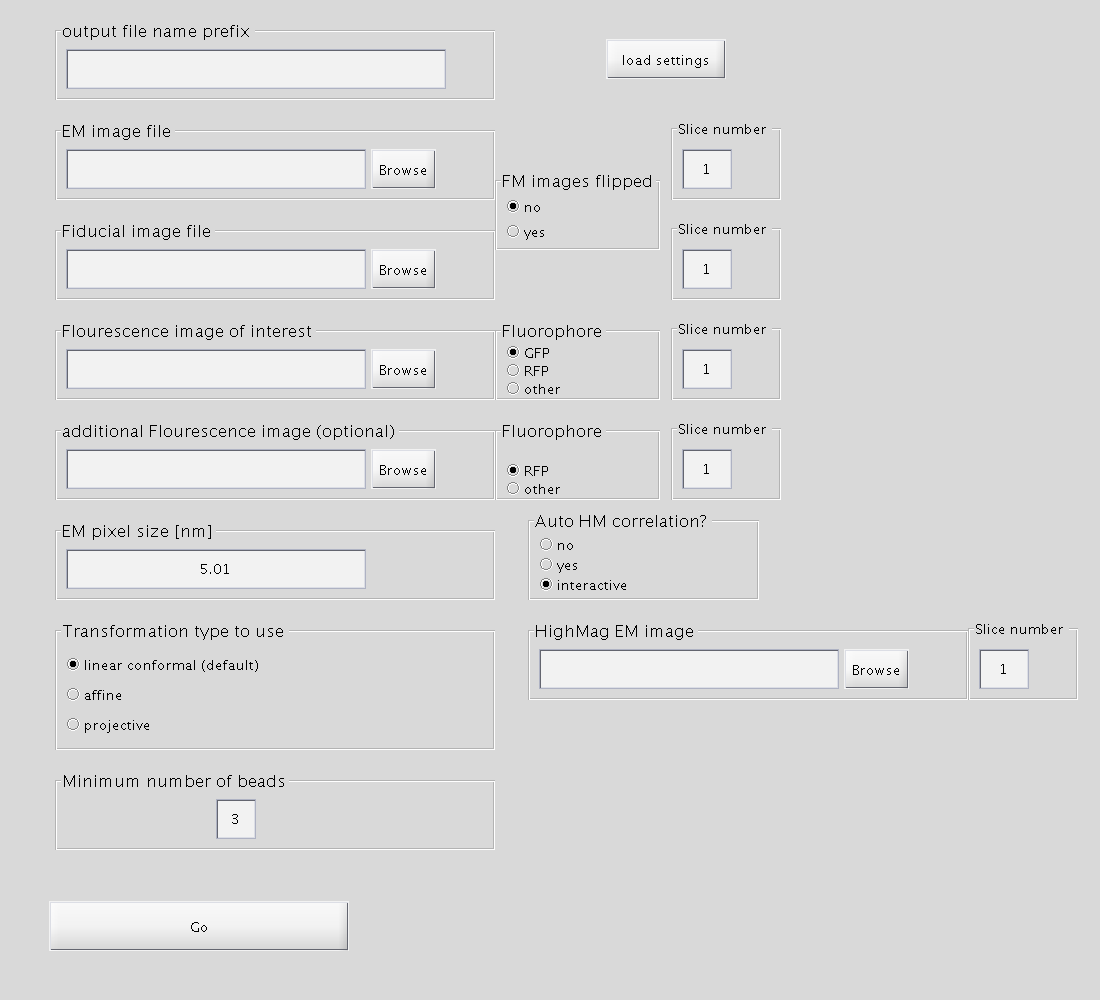
\includegraphics[width=0.75\textwidth]{images/corr_gui}
 \caption{Initialization dialog}
 \label{fig:init-gui}
\end{figure}

\subsubsection{Contrast adjustment - optional}
If selected in the initialization script, the contrast of each fluorescent image can be adjusted. This is done using the script \verb|martin_contrast(image)|. The contrast can be adjusted either manually or automatically.

\begin{figure}[h!]
 \centering
 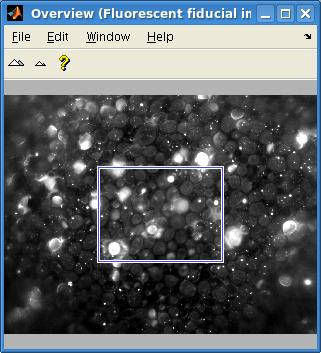
\includegraphics[width=0.2\textwidth]{images/contr_overview.jpg}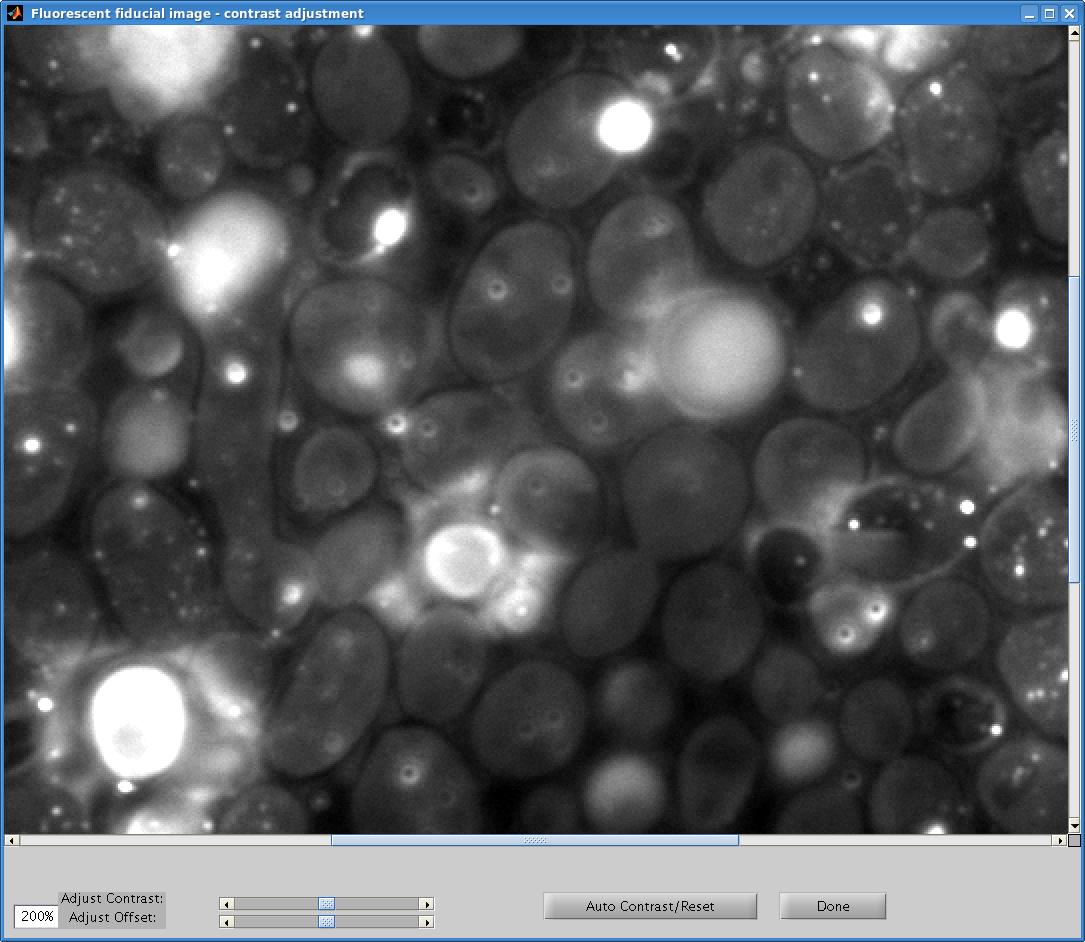
\includegraphics[width=0.6\textwidth]{images/contr.jpg}
 % contr.jpg: 1085x942 pixel, 762dpi, 3.62x3.14 cm, bb=0 0 103 89
 \caption{Contrast adjustment tool}
 \label{fig:contrast}
\end{figure}

A file selection dialog will ask to open already existing fiducial coordinate files. If the selected images have never been used for correlating before, just close that window.\\

\subsubsection{Rotation of the fluorescence fiducial image}
\label{sec:rotation}

If no previous fiducial coordinates could be found you can rotate the fluorecence fiducial image in 90 degree steps to simplify the initital detection of fiducial pairs.\,(Fig.\,\ref{fig:rotate}) Just rotate the image until its orientation fits best the EM-image presented in the small window.

\begin{figure}[h]
 \centering
 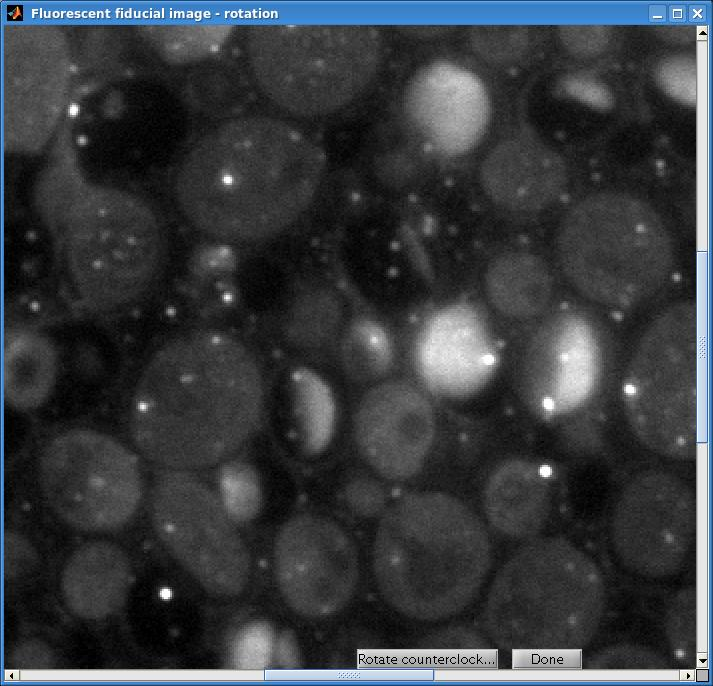
\includegraphics[width=0.5\textwidth]{images/rotate.jpg}
 % rotate.jpg: 713x686 pixel, 762dpi, 2.38x2.29 cm, bb=0 0 67 65
 \caption{Image rotation window for initial correlation}
 \label{fig:rotate}
\end{figure}

If the proper orientation is selected, click ``Done''. The initial manual assignment of fiducial pairs now is done with the selected orientation. For the further processing and coordinate checks the original orientation will be used.


\subsubsection{Fiducial selection}
\label{sec:fiducials}

Fiducial pairs are selected in both LM and EM image using the \texttt{cpselect} tool. When an already existing coordinate file is opened, these are displayed.\, (Fig.\,\ref{fig:cpsel_fid1}) To continue, close the window.

\begin{figure}[ht!]
 \centering
 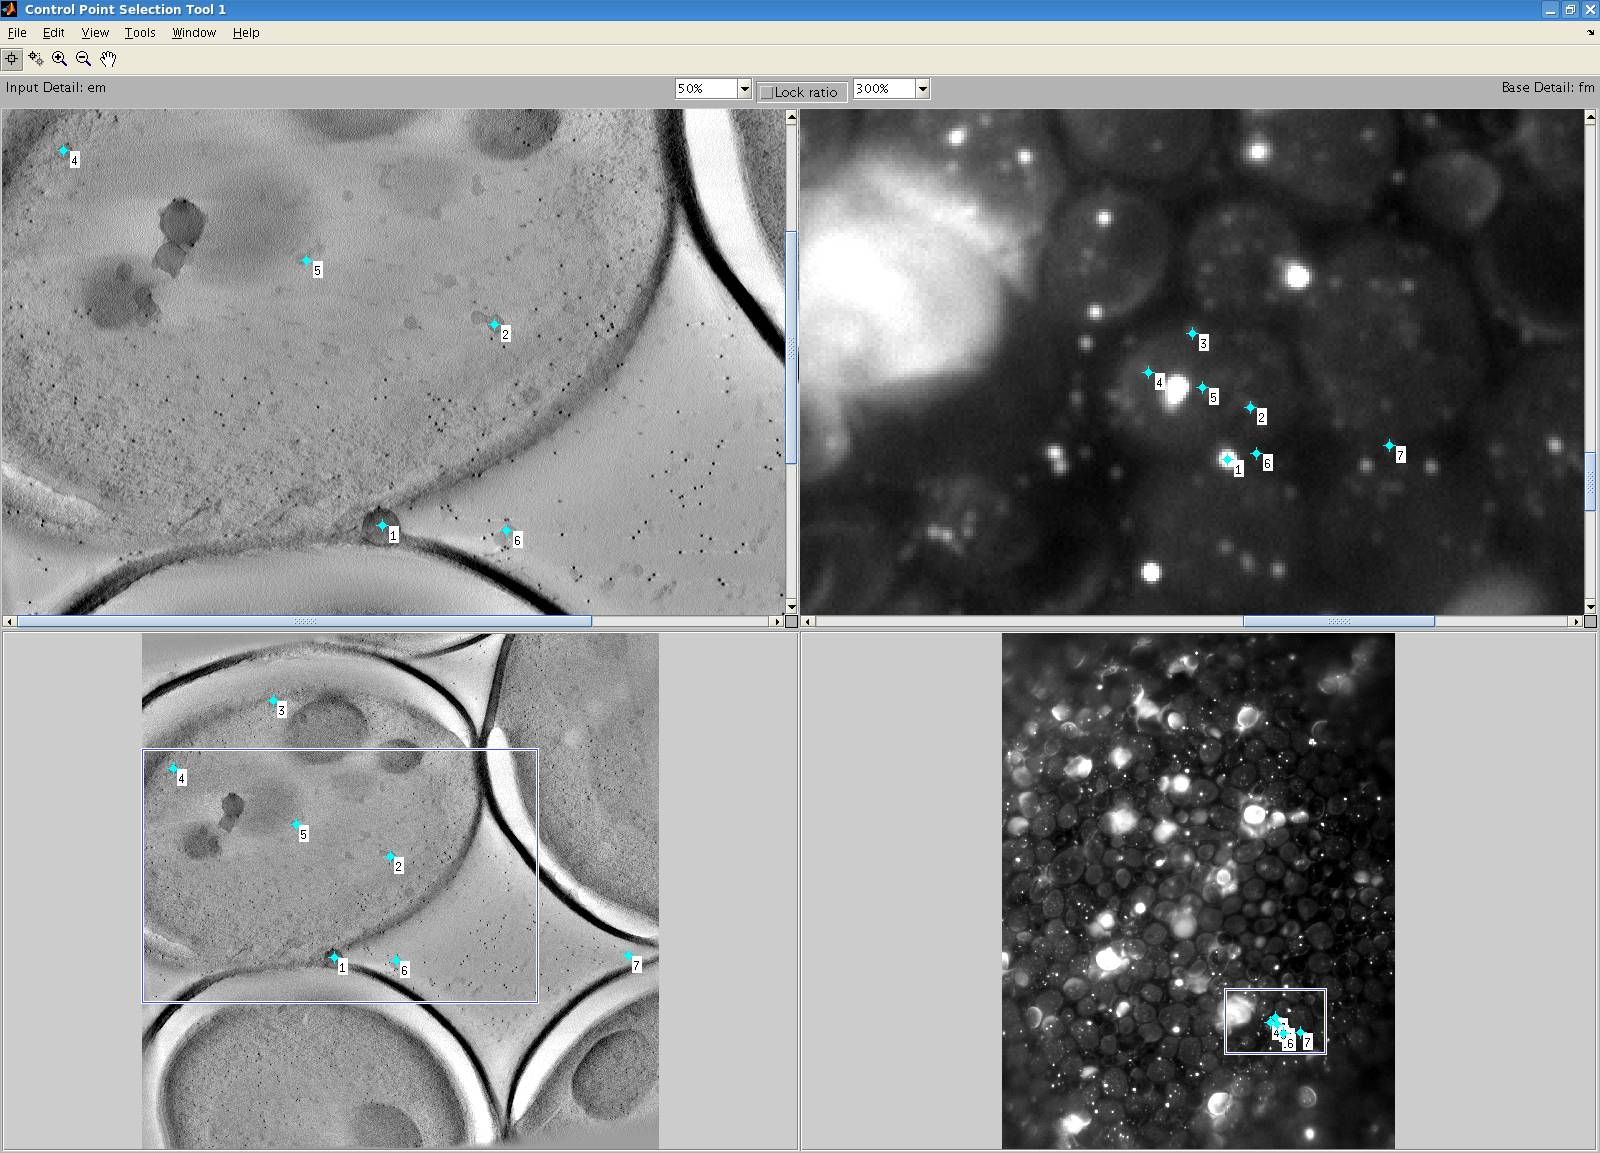
\includegraphics[width=.83\textwidth]{images/cpsel_fid1.jpg}
 % cpsel_fid1.png: 1600x1153 pixel, 72dpi, 56.44x40.68 cm, bb=0 0 1600 1153
 \caption{\texttt{cpselect} -- graphical interface for picking and checking fiducial positions}
 \label{fig:cpsel_fid1}
\end{figure}

\subsubsection{Fiducial sub-pixel fitting and display}
\label{sec:gaussfit}
Fiducial positions in the light microscopy image are fitted with sub-pixel accuracy using a  2D Gaussian fit \texttt{martin\_2dgaussfit}.
You can specify in the init file that you want to check the fit and adjust each fiducial pair individually.

If intersctive fitting is desired, a window showing the fit (Fig.\,\ref{fig:gaussfit_gui}) is presented for each of the beads. The fitted 2D-Gaussian is shown as black mesh on top of the pixel intensity visualized as a surface plot. The initially clicked position is indicated by the magenta vertical line. The following options are possible:
\begin{itemize}
 \item 'keep fit' -- use the fitted coordinates
 \item 'keep original' -- use the original clicked coordinates without fit
 \item 'select manually' -- a \texttt{cpselect} dialog showing the detailed region opens and allows you to further specify the location of the spot. Change the position of the point 1 in one of the windows (the one where the contrast fits best) and close the dalog. Then the identical fitting procedure is run on a smaller cropped region of the image around the chosen coordinates.
 \item 'redo fit' -- the fit is done again using a different preset for the subtraction of linear background
 \item 'kick out points' -- the current fiducial pair is removed from the dataset
\end{itemize}

\begin{figure}[h!]
 \centering
 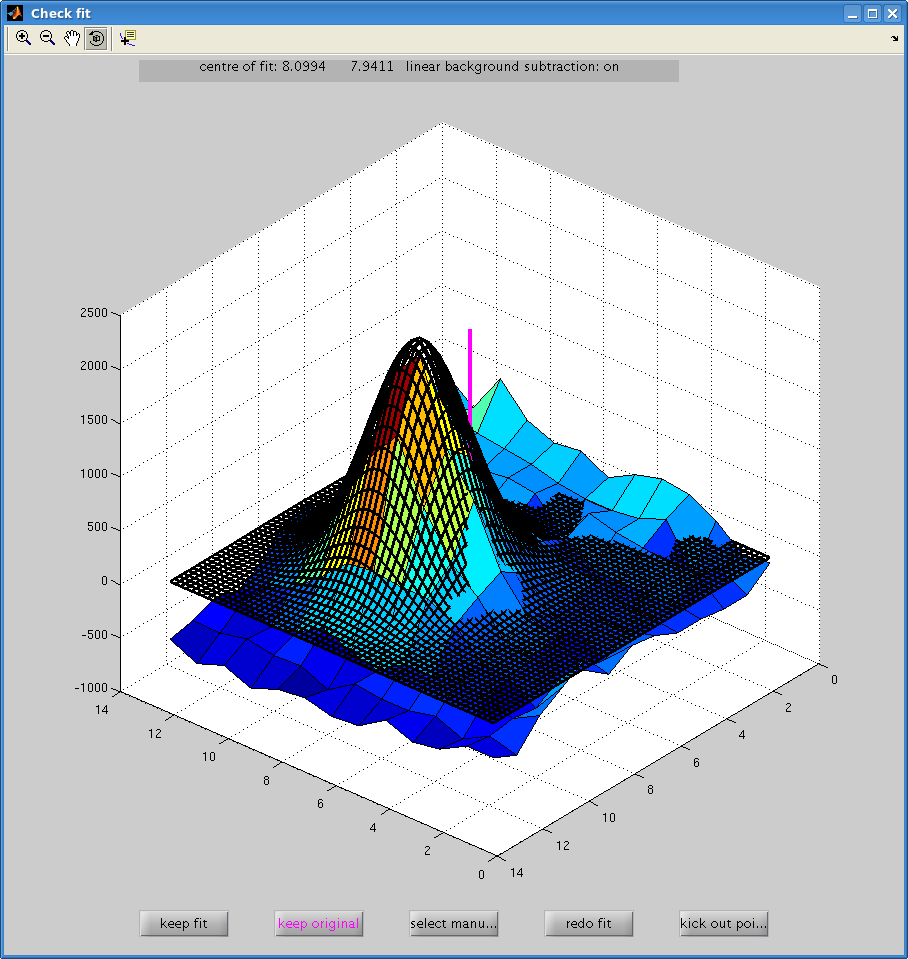
\includegraphics[width=0.65\textwidth]{images/gaussfit_gui.png}
 % gaussfit_gui.png: 908x959 pixel, 72dpi, 32.03x33.83 cm, bb=0 0 908 959
 \caption{Interactive check of the sub-pixel fitting}
 \label{fig:gaussfit_gui}
\end{figure}


The fitted positions are presented again using a \texttt{cpselect} dialog.\,(Fig.\,\ref{fig:cpsel_fid1}) To continue, close the window.




 \lstinputlisting[linerange={167-169,180-181}]{../martin_correlate.m}

% \subsubsection{Selection of fluorescence channel}
% A popup window will ask you to determine the fluorescence channel in which your signal of interest is imaged.(Fig.\,\ref{fig:fluorsel})
% 
% \begin{figure}
%  \centering
%  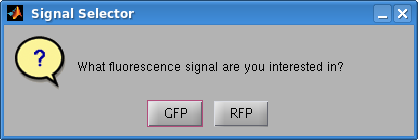
\includegraphics[width=.38\textwidth]{images/fluorsel.png}
%  % fluorsel.png: 418x140 pixel, 72dpi, 14.75x4.94 cm, bb=0 0 418 140
% \caption{graphical interface for selecting the fluorescence channel}
%  \label{fig:fluorsel}
% \end{figure}

\subsubsection{Picking the fluorescent spot(s) of interest}
In the folowing \texttt{cpselect} dialog, the selected fluorescence image is shown on the right, the positions indicating the fiducial markers. Click once in the right image to determine the position of the spot of interest AND once in the left image just anywhere. This click in the left image will have no effect on the correlation. \texttt{cpselect} otherwise would just not export the clicked coordinates.\,(Fig.\,\ref{fig:cpsel_fluor1}) To continue, close the window. In case you forget to click in the left image, a reminder will be shown and you have the chance to click again. 

When choosing the \texttt{multispot} option you have to select a pair of coordinates for each of the spots of interest. You can double check the intended number of spots with the clicks captured by the program.
\begin{figure}
 \centering
 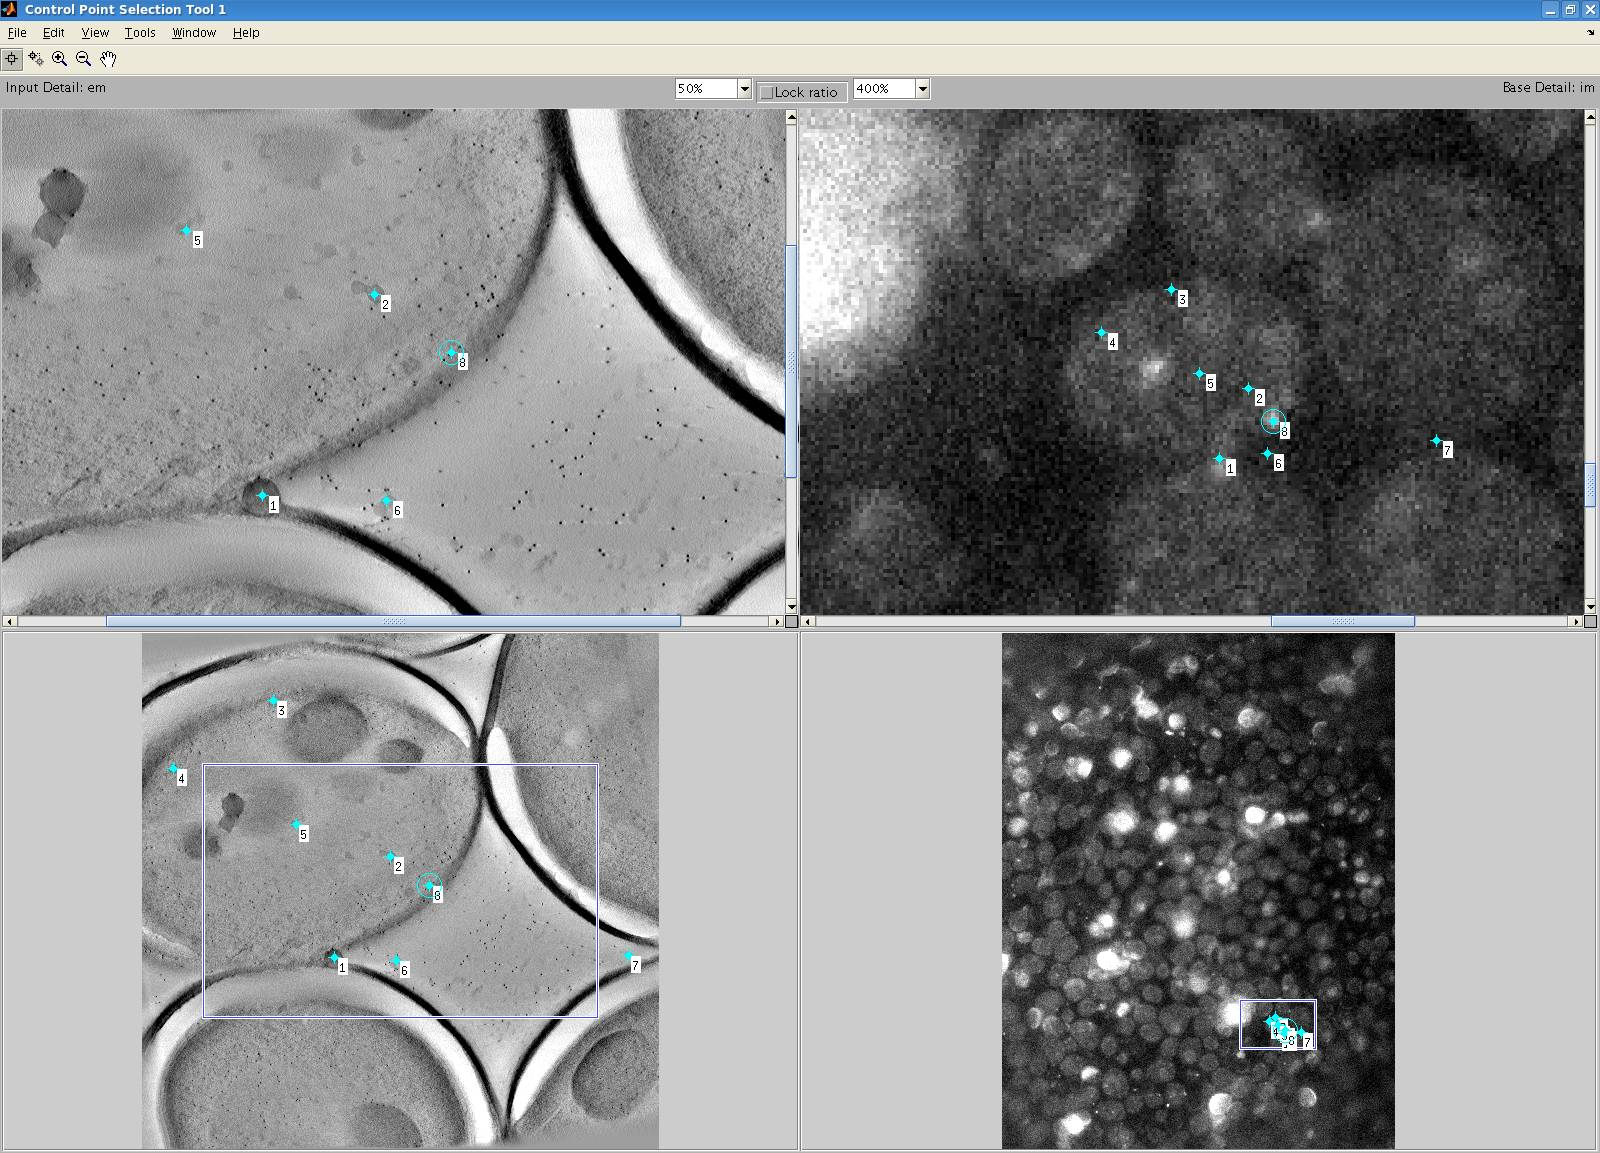
\includegraphics[width=.78\textwidth]{images/cpsel_fluor1.jpg}
 % cpsel_fluor1.png: 1600x1153 pixel, 72dpi, 56.44x40.68 cm, bb=0 0 1600 1153
 \caption{Selection of the fluorescent spot of interest -- marked spots with nubers \#8. The selected fluorescence channel image is shown on the right, the left click can be arbitrary in position.}
 \label{fig:cpsel_fluor1}
\end{figure}

\subsubsection{Sub-pixel fitting of the fluorescent spot(s) of interest}
The coordinates of the fluorescent spot(s) of interest are also determined by a gaussian fit of the image. (For details see \ref{sec:gaussfit}, Fig.\,\ref{fig:gaussfit_gui}) The resulting coordinate(s) will be presented in a new \texttt{cpselect} window. (Fig.\,\ref{fig:cpsel_fluor2})\\

To continue, close the window. 

\lstinputlisting[linerange={294-296,300-301}]{../martin_correlate.m}

\begin{figure}
 \centering
 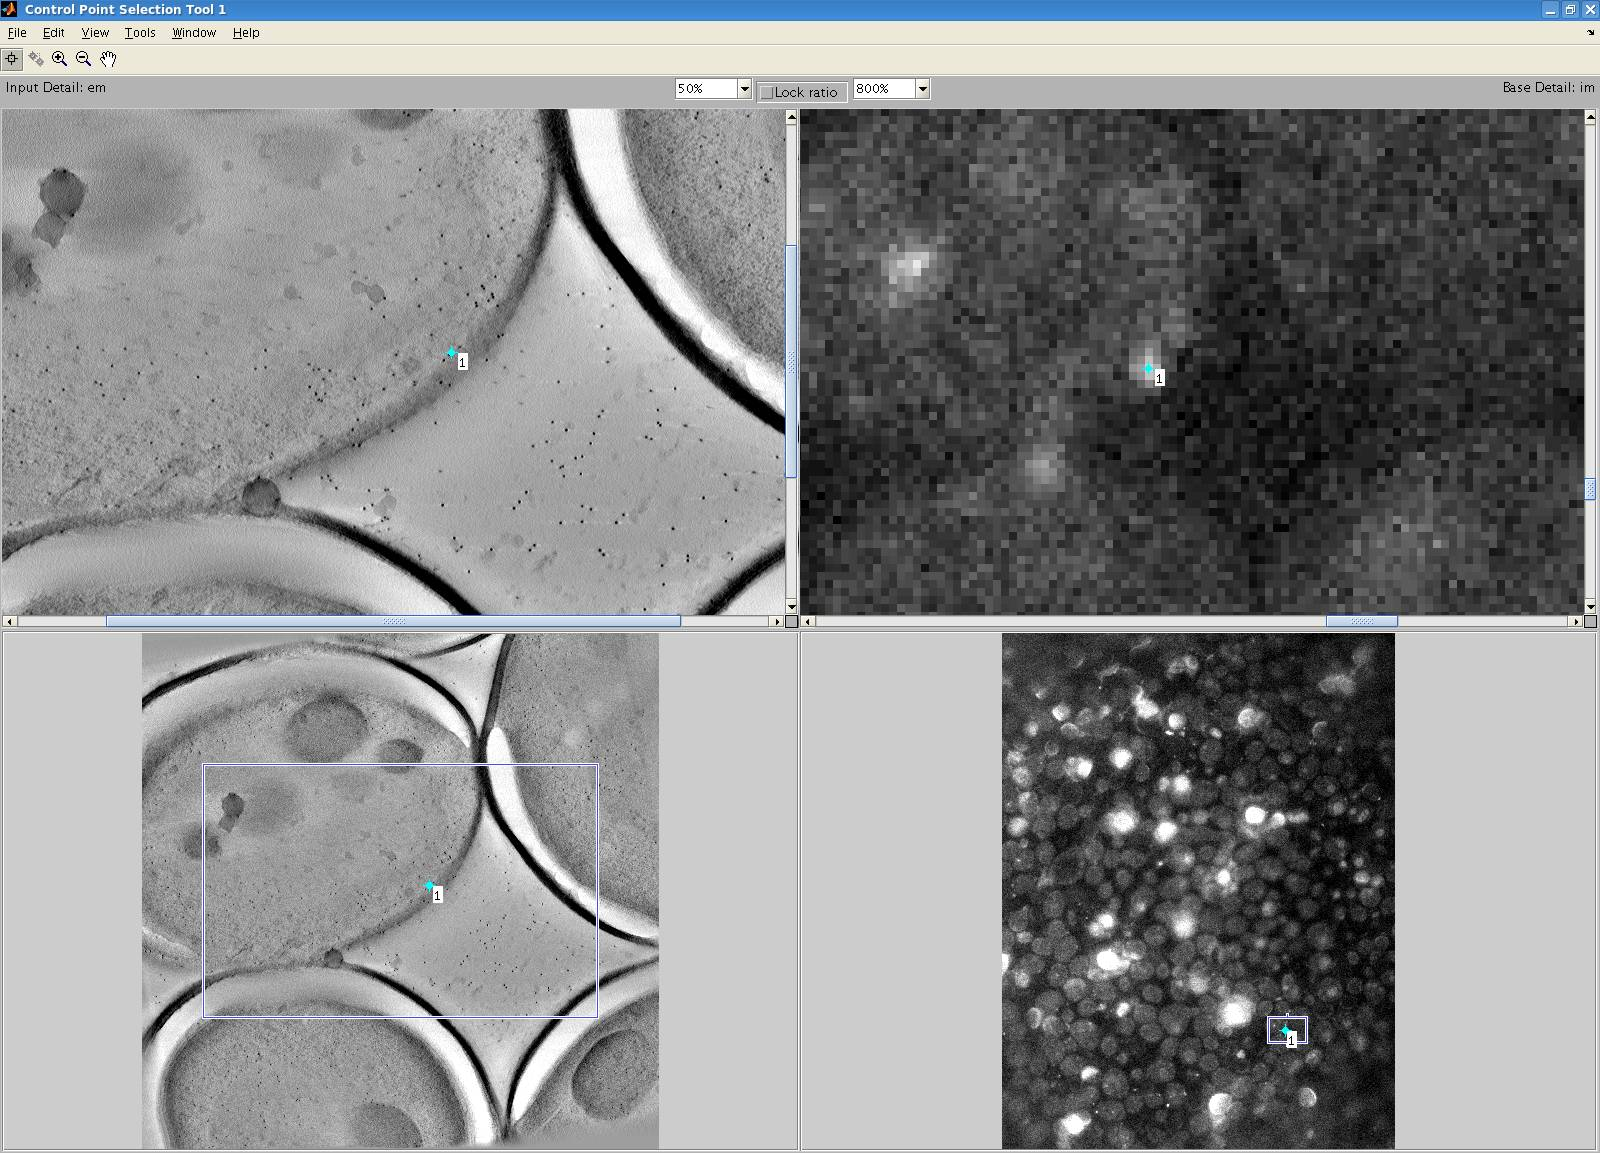
\includegraphics[width=.78\textwidth]{images/cpsel_fluor2.jpg}
 % cpsel_fluor2.png: 1600x1153 pixel, 72dpi, 56.44x40.68 cm, bb=0 0 1600 1153
 \caption{Positioning of the spot(s) of interest after sub-pixel fitting.}
 \label{fig:cpsel_fluor2}
\end{figure}

\subsubsection{Correction of stage drift in between imaging of the different fluorescence channels}
The possible drift of the light microscope stage in between acquisition of the different flourescence images is accounted for using the fiducial signal that bleeds through into the longer wavelength channels. This step can be skipped if not needed by. Just close the selection window and select ``Export and Close''. To continue then press any key while having the main MATLAB window active. If you constantly want to skip this correction you can modify your configuration script accordingly.\\

A file selection window will ask for already existing files storing these coordinates.\\

In case no pre-existing shift coordinates are selected a new window will open showing an RGB-overlay of the fiducial fluorescence image in red and the selected fluorescence channel containing the signal of interest in green. (Fig.\,\ref{fig:digitize})
Click the obvious bleeding fiducials (both channels show a spot-like signal in close proximity) and close the window, saving the positions. The entire shift correction procedure is done by:
\lstinputlisting[linerange={339-339}]{../martin_correlate.m}
If you cannot find any obvious points, just continue without clicking postitions. The shift correction will then be skipped.\\

To continue press any key while having the main MATLAB window active.\\

\begin{figure}
 \centering
 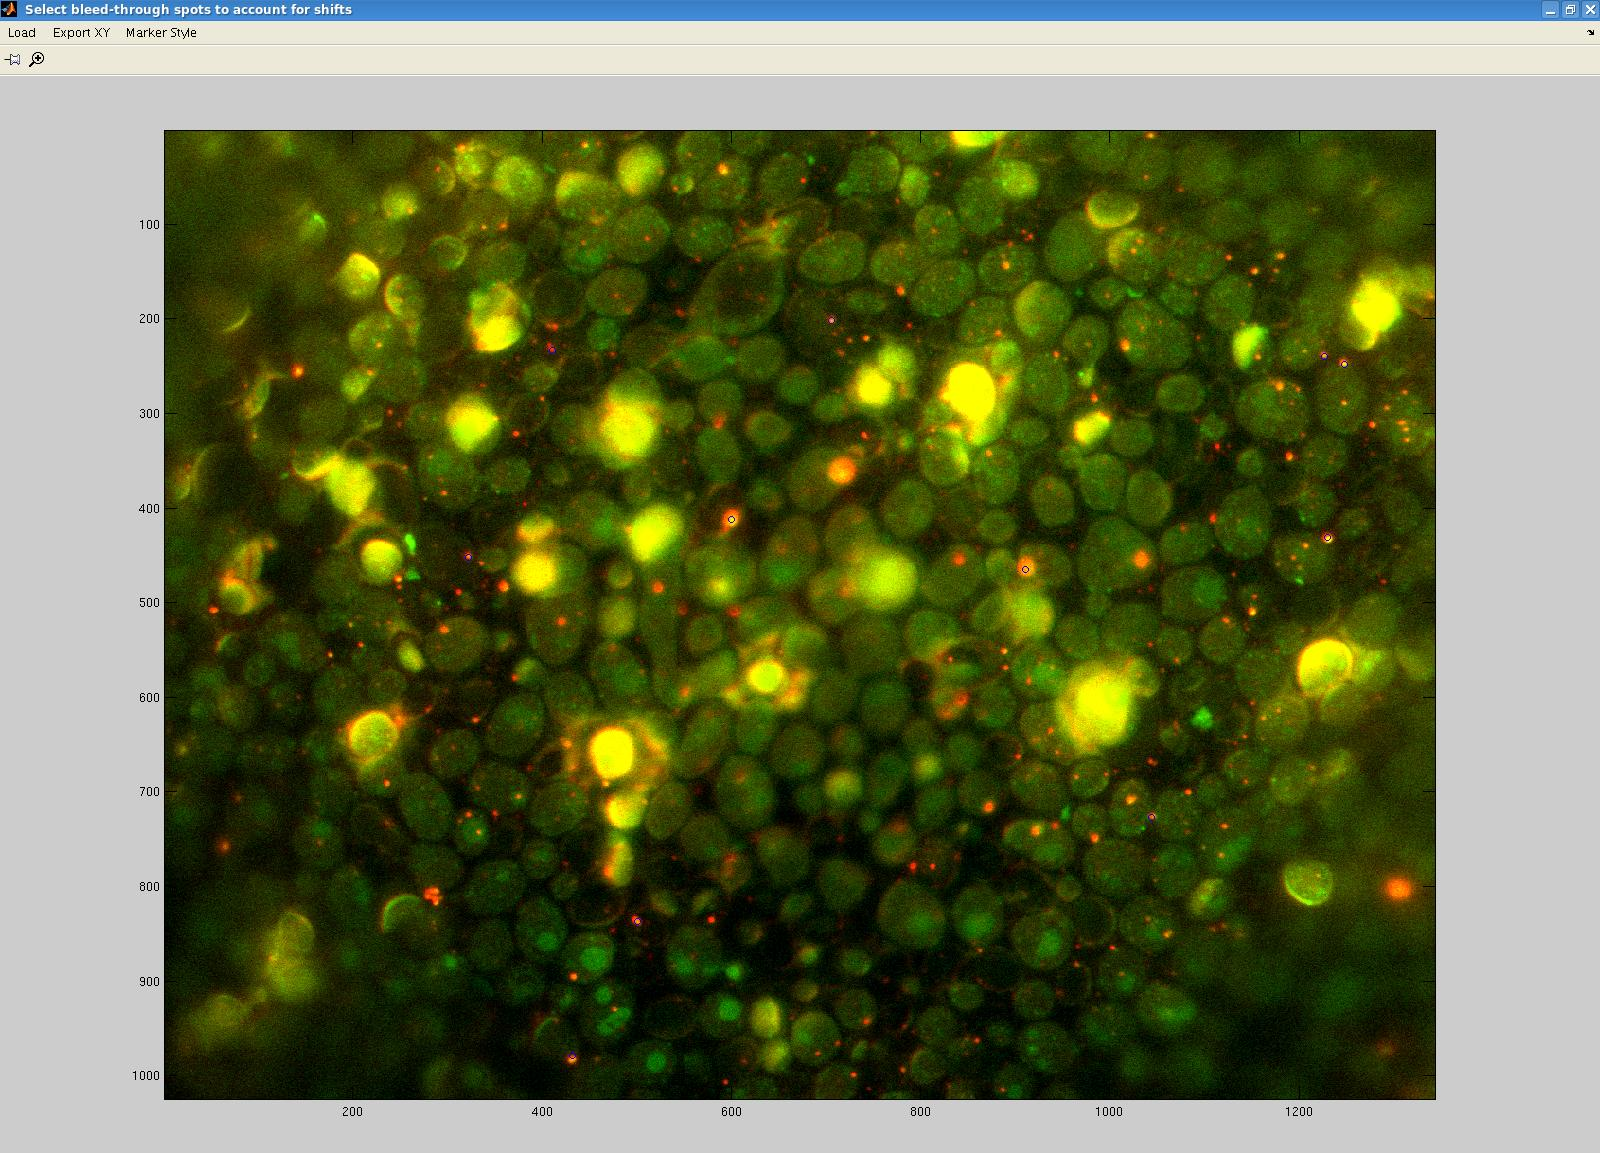
\includegraphics[width=.75\textwidth]{images/digitize.jpg}
 % digitize.jpg: 1600x1153 pixel, 762dpi, 5.33x3.84 cm, bb=0 0 151 109
 \caption{The tool for selecting the fiducials bleeding through to the fluorescence channel of interest. Clicked positions are indicated using blue circles.}
 \label{fig:digitize}
\end{figure}

\subsubsection{Calculation of the optimal transform and predicting fiducial and fluorescent spot EM-coordinates.}
Based on the set of clicked fiducials, the most accurate linear transformation (consisting of scaling, a translation and a rotation) of coordinates is calculated using the script \texttt{martin\_tfm\_beads}.
\lstinputlisting[linerange={407-408}]{../martin_correlate.m}

% It scores the transformation based on all beads with the optimal transformation obtained by using a subset of beads omitting each selected fiducial pair once by comparing the sum of squares of the deviation from the predicted position of all beads with the clicked position in the EM-image.
% $$
% \epsilon = \frac{1}{N}\sum_{i=1}^N (T({x_{FM_i}})-x_{EMclicked_i})^2
% $$
% \lstinputlisting[linerange={410-411}]{../martin_correlate.m}

The resulting best coordinate transformation is applied to all cordinates and presented in a graphical output window. (Fig.\,\ref{fig:tfm_select}) The beads chosen for the transformation are displayed in the bottom left. Blue positions show the clicked coordinates in the EM-image, green dots represent the transformed position of corresponding fiducial signal from the fluorescence image. To have an idea where the spot of interest is predicted, it is shown by a magenta circle. By clicking the lower button, obiously mispicked beads can be corrected, jumping to the selection step of the algorithm.(\ref{sec:fiducials}) When clicking ``GO'', all output files will be created using the presented coordinate transformation.\\
An overlay image showing the predicted spot(s) within the EM image as a white circle (Fig.\,\ref{fig:tfm_appl}) indicates a successful run of the collelating sript.
\begin{figure}
 \centering
 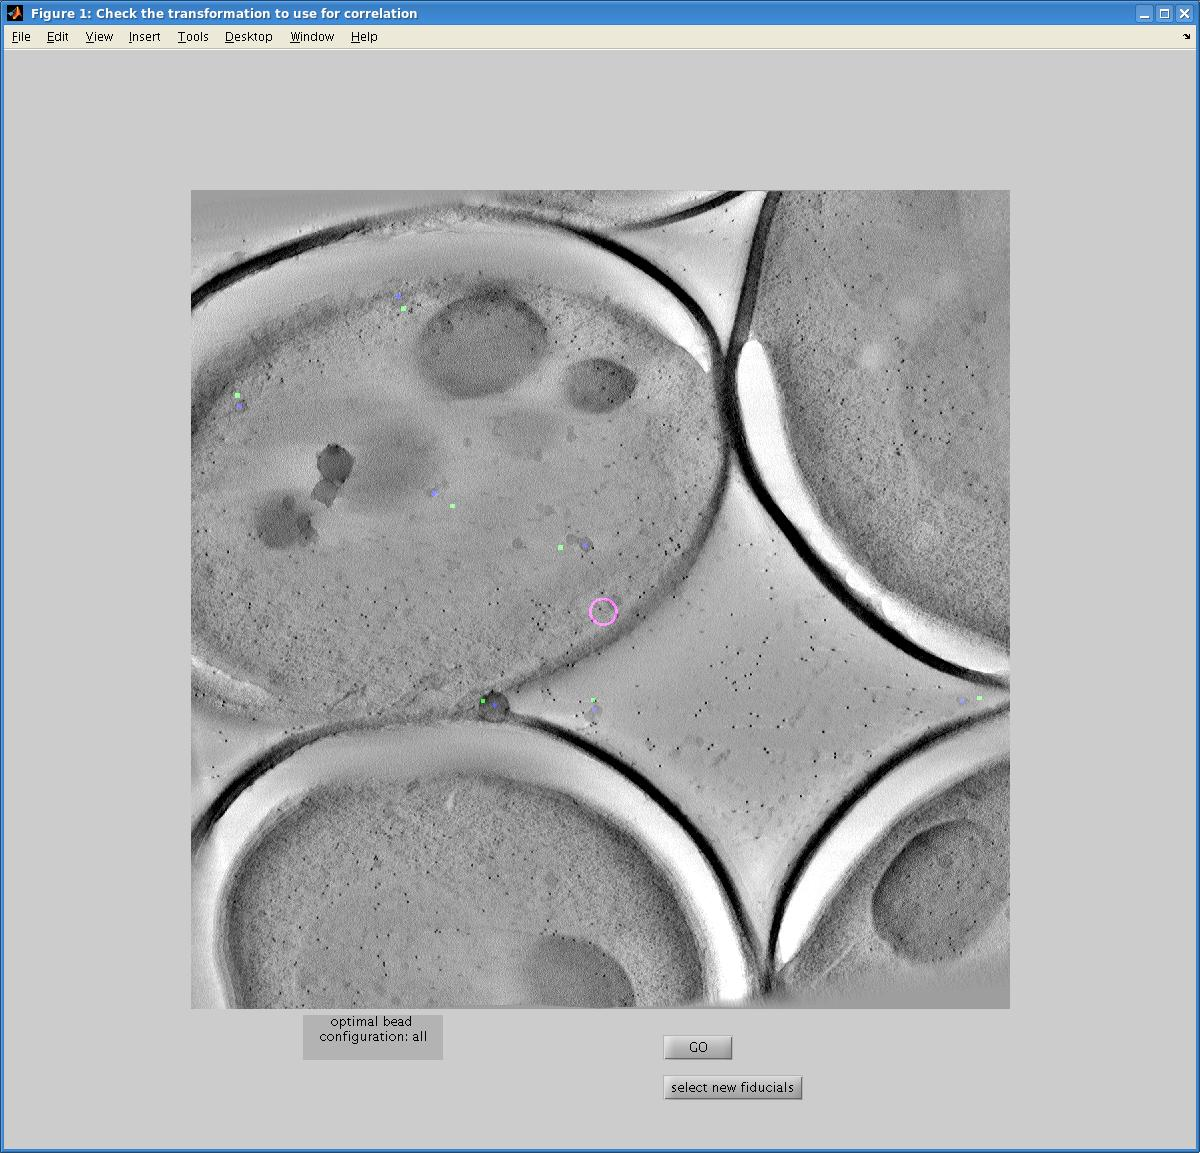
\includegraphics[width=.7\textwidth]{images/tfm_select.jpg}
 % tfm_select.jpg: 1200x1153 pixel, 762dpi, 4.00x3.84 cm, bb=0 0 113 109
 \caption{Preview of the coordinate transform. Fiducial selection can be modified by clicking the lower button.}
 \label{fig:tfm_select}
\end{figure}

\begin{figure}
 \centering
 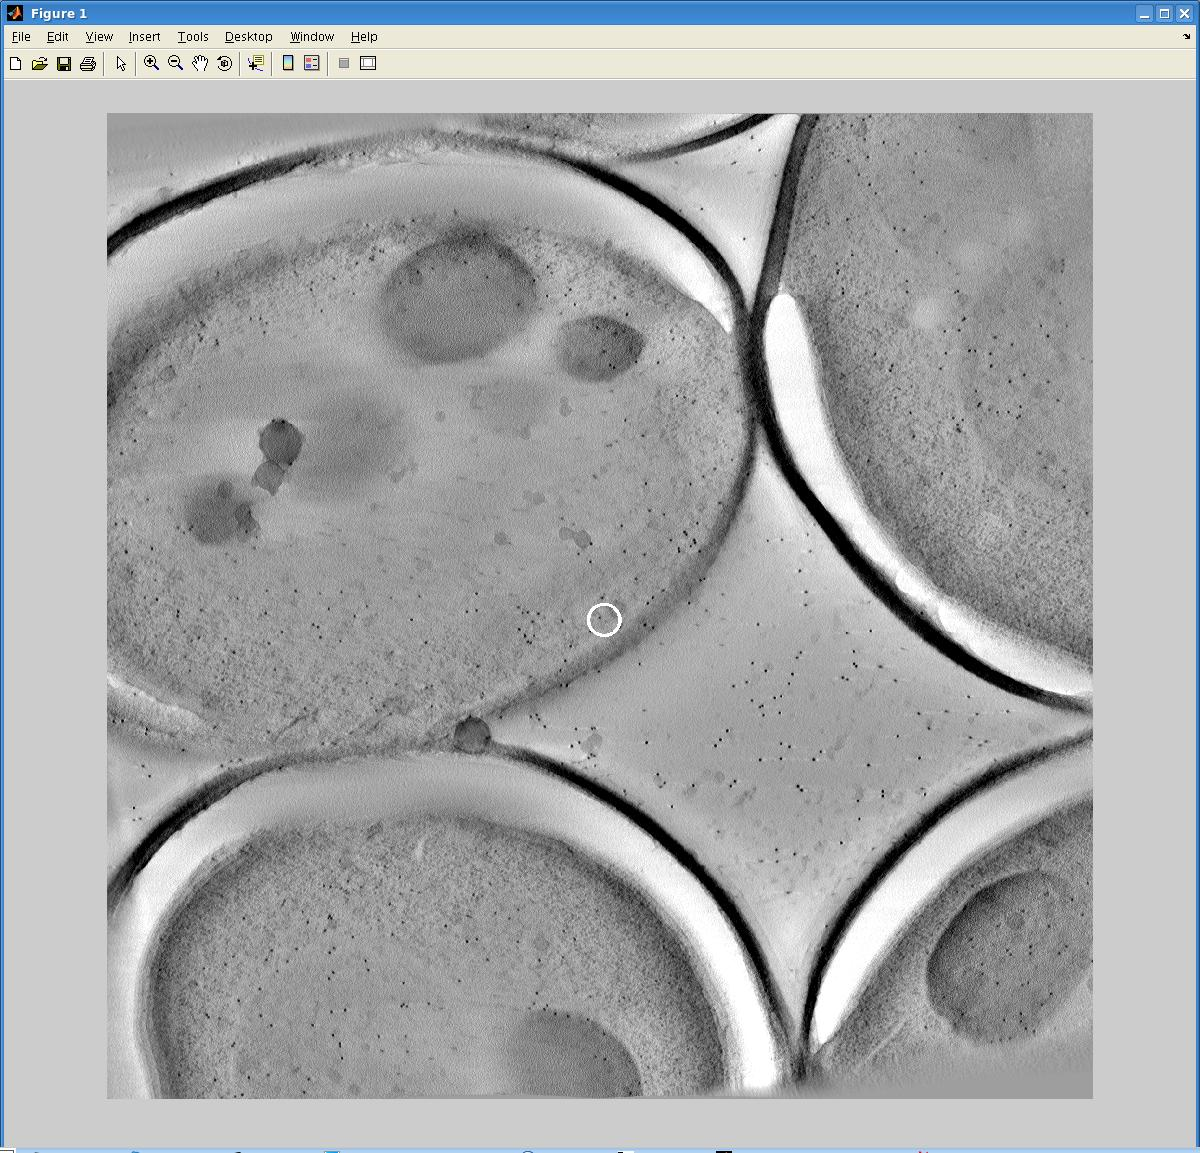
\includegraphics[width=.7\textwidth]{images/tfm_appl.jpg}
 % tfm_appl.jpg: 1200x1153 pixel, 762dpi, 4.00x3.84 cm, bb=0 0 113 109
 \caption{Performed correlation. Output position indicated by the white circle overlay.}
 \label{fig:tfm_appl}
\end{figure}

 \newpage
\section{Correlation form low magnification tomogram to high magnification EM image}

Correlation from a low resolution EM tomogram slice to a high magnification image of the same sample containing indentifiable fiducial markers such as the gold beads used for tomogram reconstruction is performed using the script \texttt{martin\_LMtoHM.m}.
\subsection{Executing the script}
To execute the script and start the correlation simply run \begin{verbatim}
 martin_LMtoHM(hmf,smf,outfileroot)
\end{verbatim}
 in the MATLAB command line.

\lstinputlisting[linerange={1-18}]{../martin_LMtoHM.m}
It requires the following input parameters:
\begin{enumerate}
 \item\texttt{hmf} -- path to high mag. electron tomogram slice containing fiducial information (usually 2048$\times$2048 pixel, 8 or 16bit tiff-file)
 \item\texttt{smf} -- path to high mag. electron tomogram slice containing a probable feature of interest that is to be checked for correlation with the fluorescence signal (usually 2048$\times$2048 pixel, 8 or 16bit tiff-file)
 \item\texttt{outfileroot} -- directory and name base for generating output files.
\end{enumerate}
\subsection{Output and generated files}
The following files are generated by the correlation script during runtime. Abbreviations of file name prefixes as in \ref{sec:lm_output}. In case you require also the transformed FM images for overlays you can activate generation of those in the config script.
\begin{itemize}
\item \texttt{BASE\_XFP\_\#\_XFP.lmhmcoos.mat} -- Coordinates of fiducial marker pairs in both EM images
\lstinputlisting[linerange={41-41}]{../martin_chromaticshift_drift2.m}

\item \texttt{BASE\_XFP\_\#\_hm.tif} -- high mag. electron tomogram slice containing fiducial information 
\item \texttt{BASE\_XFP\_\#\_sm.tif} -- high mag. electron tomogram slice containing the probable feature of interest 
\item \texttt{BASE\_XFP\_\#\_XFP\_hm\_prd\_overlay.tif} -- Overlay of the prediction circle and high mag EM image containing the probable feature.


\item \texttt{BASE\_XFP\_\#\_\_XFP\_hm\_transform.log} -- Plain text log file containing the source files used for correlation, the transformed spot coordinates and information about the used transformation
\end{itemize}
\newpage
\subsection{User interaction and key procedures}
\subsubsection{Fiducial selection}
\label{sec:HM_fiducials}
A file selection dialog will ask to open the data file created by the initial correlation of the fluorescence signal.(\texttt{BASE\_XFP\_\#.appltfm.mat}) Here you have to provide a file, otherwise the script obviously cannot transform the coordinates.% After that you are asked to confirm the fluorescence channel of interest.
A file selection dialog will ask to open already existing fiducial coordinate files for the current lowMag to highMag correlation. If the selected images have never been used for correlating before, just close that window.\\

Fiducial pairs are selected in both LM and HM image using the \texttt{cpselect} tool. When an already existing coordinate file is opened, these are displayed. (Fig.\,\ref{fig:cpsel_HM}) To continue, close the window.
\begin{figure}
 \centering
 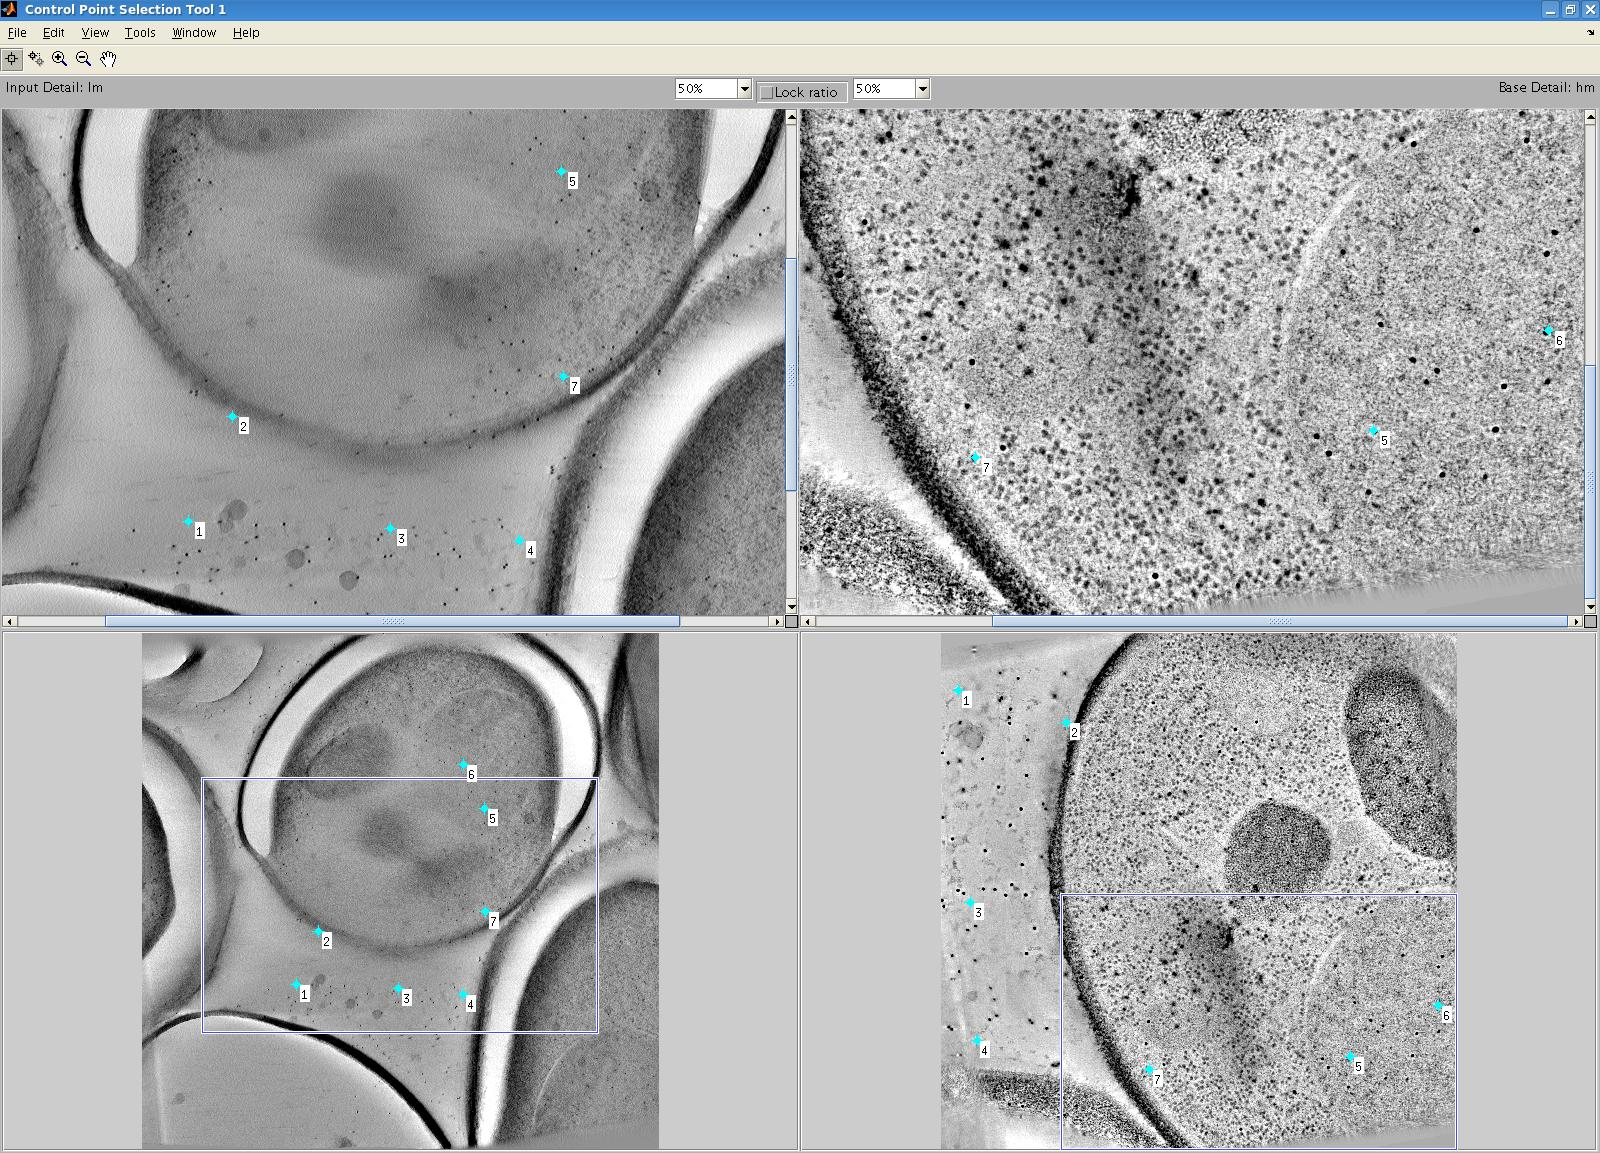
\includegraphics[width=.78\textwidth]{images/cpsel_HM.jpg}
 % cpsel_HM.jpg: 1600x1153 pixel, 72dpi, 56.44x40.68 cm, bb=0 0 1600 1153
 \caption{\texttt{cpselect} -- graphical interface for picking and checking fiducial positions}
 \label{fig:cpsel_HM}
\end{figure}
% \subsubsection{Fiducial sub-pixel fitting and display}
% Fiducial positions both image are fitted with sub-pixel accuracy using a center of mass detection.
% The fitted positions are presented again using a \texttt{cpselect} dialog. To continue, close the window.

\subsubsection{Correlation}
Coordinates are transformed using all marked fiducials and the output files are written. An overlay image showing the predicted spot within the highMag image containing the feature of interest (Fig.\,\ref{fig:tfm_HM}) indicates a successful run of the collelating sript.
\begin{figure}[h!]
 \centering
 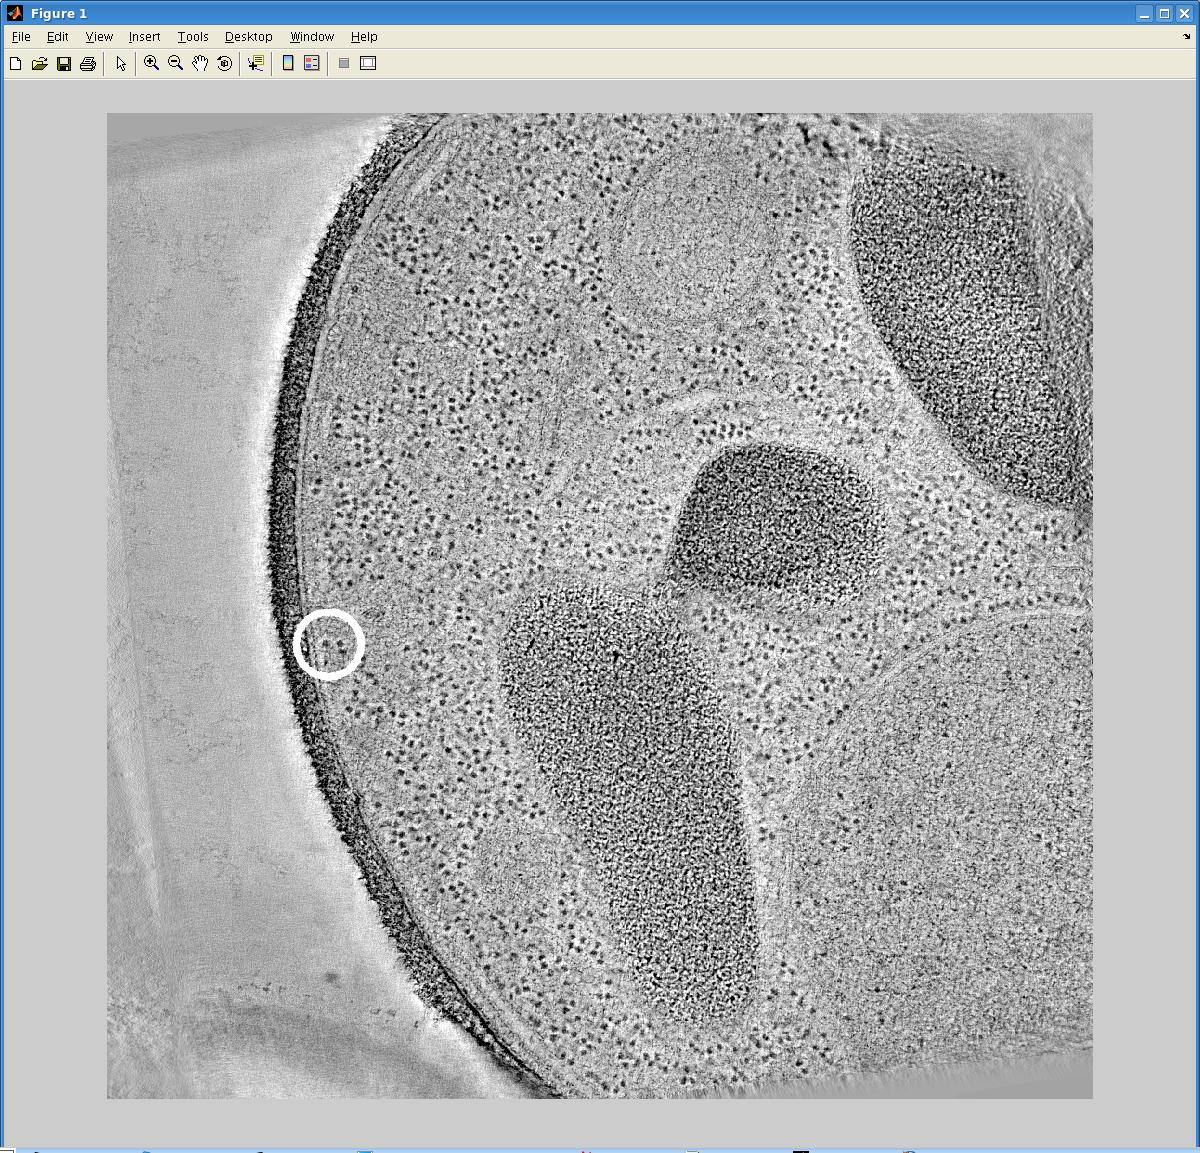
\includegraphics[width=.5\textwidth]{images/tfm_HM.jpg}
 % tfm_HM.jpg: 1200x1153 pixel, 762dpi, 4.00x3.84 cm, bb=0 0 113 109
 \caption{Performed correlation. Output position indicated by the white circle overlay.}
 \label{fig:tfm_HM}
\end{figure}
\newpage
% \section{Accuracy determination}
% The accuracy of a set of correlations performed on a certain kind of sample can be estimated by calculating the deviation of a transformed fluorescence signal of a fiducial with its true position in the EM image. The transformation is therefore generated using the remaining beads out of the set of fiducials.
% 
% Once you have run a reasonable number of correlations you can use the following procedure to determine the accuracy. It is crucial that all the EM images you used for the correlations are of the same pixel size in order to compare the deviations.
% 
% 



\newpage
\section{Useful hints and tricks}
\subsection{Overlay of correlated images}
The correlation procedure writes a variety of images in tiff format that have all be aligned to each other according to the transformation used for correlation. (see\,\ref{sec:lm_output}) These include transformed fluorescence images as well as prediction circles or fiducial positions.
You can easily superimpose these images to the EM image or even the tomogram.

\subsubsection*{ImageJ (version$>$1.41)}
Open both the EM image and the image you want to superimpose in ImageJ/Fiji. In Image$>$Color$>$Merge Channels select the colour channel of choice for the overlay(s) and grey for the EM image. You can then adjust the contrast for each channel by selecting the colour using the mouse wheel or the slider at the bottom of the image and the contrast adjustment tool.

\subsubsection*{Amira}
Open your original tomogram (beware of the file format issue in Amira) and create an OrthoSlice. Make sure the perspective is set to parallel. This can be done by clicking the tool button showing an eye and either parallel or diverging beams. 
\includegraphics[width=0.03\textwidth]{images/perspective.png}\\Open the image you want to superimpose, accept the parameters suggested (voxel size should be 1,1,1) and create an OrthoSlice. Select the transparency to alpha. If you want you can also adjust the color mapping. 


\end{document}